\documentclass{article}

\usepackage{graphicx}
\usepackage{tikz}
\usepackage{tikzsymbols}
\usetikzlibrary{calc,patterns,shapes.geometric}
\pagestyle{empty}
\usepackage[margin=0pt]{geometry}
\geometry{papersize={14in,12in}}

\def\centerarc[#1](#2)(#3:#4:#5){\draw[#1] ($(#2)+({#5*cos(#3)},{#5*sin(#3)})$) arc (#3:#4:#5);}

\begin{document}
	\begin{figure}
		\centering
		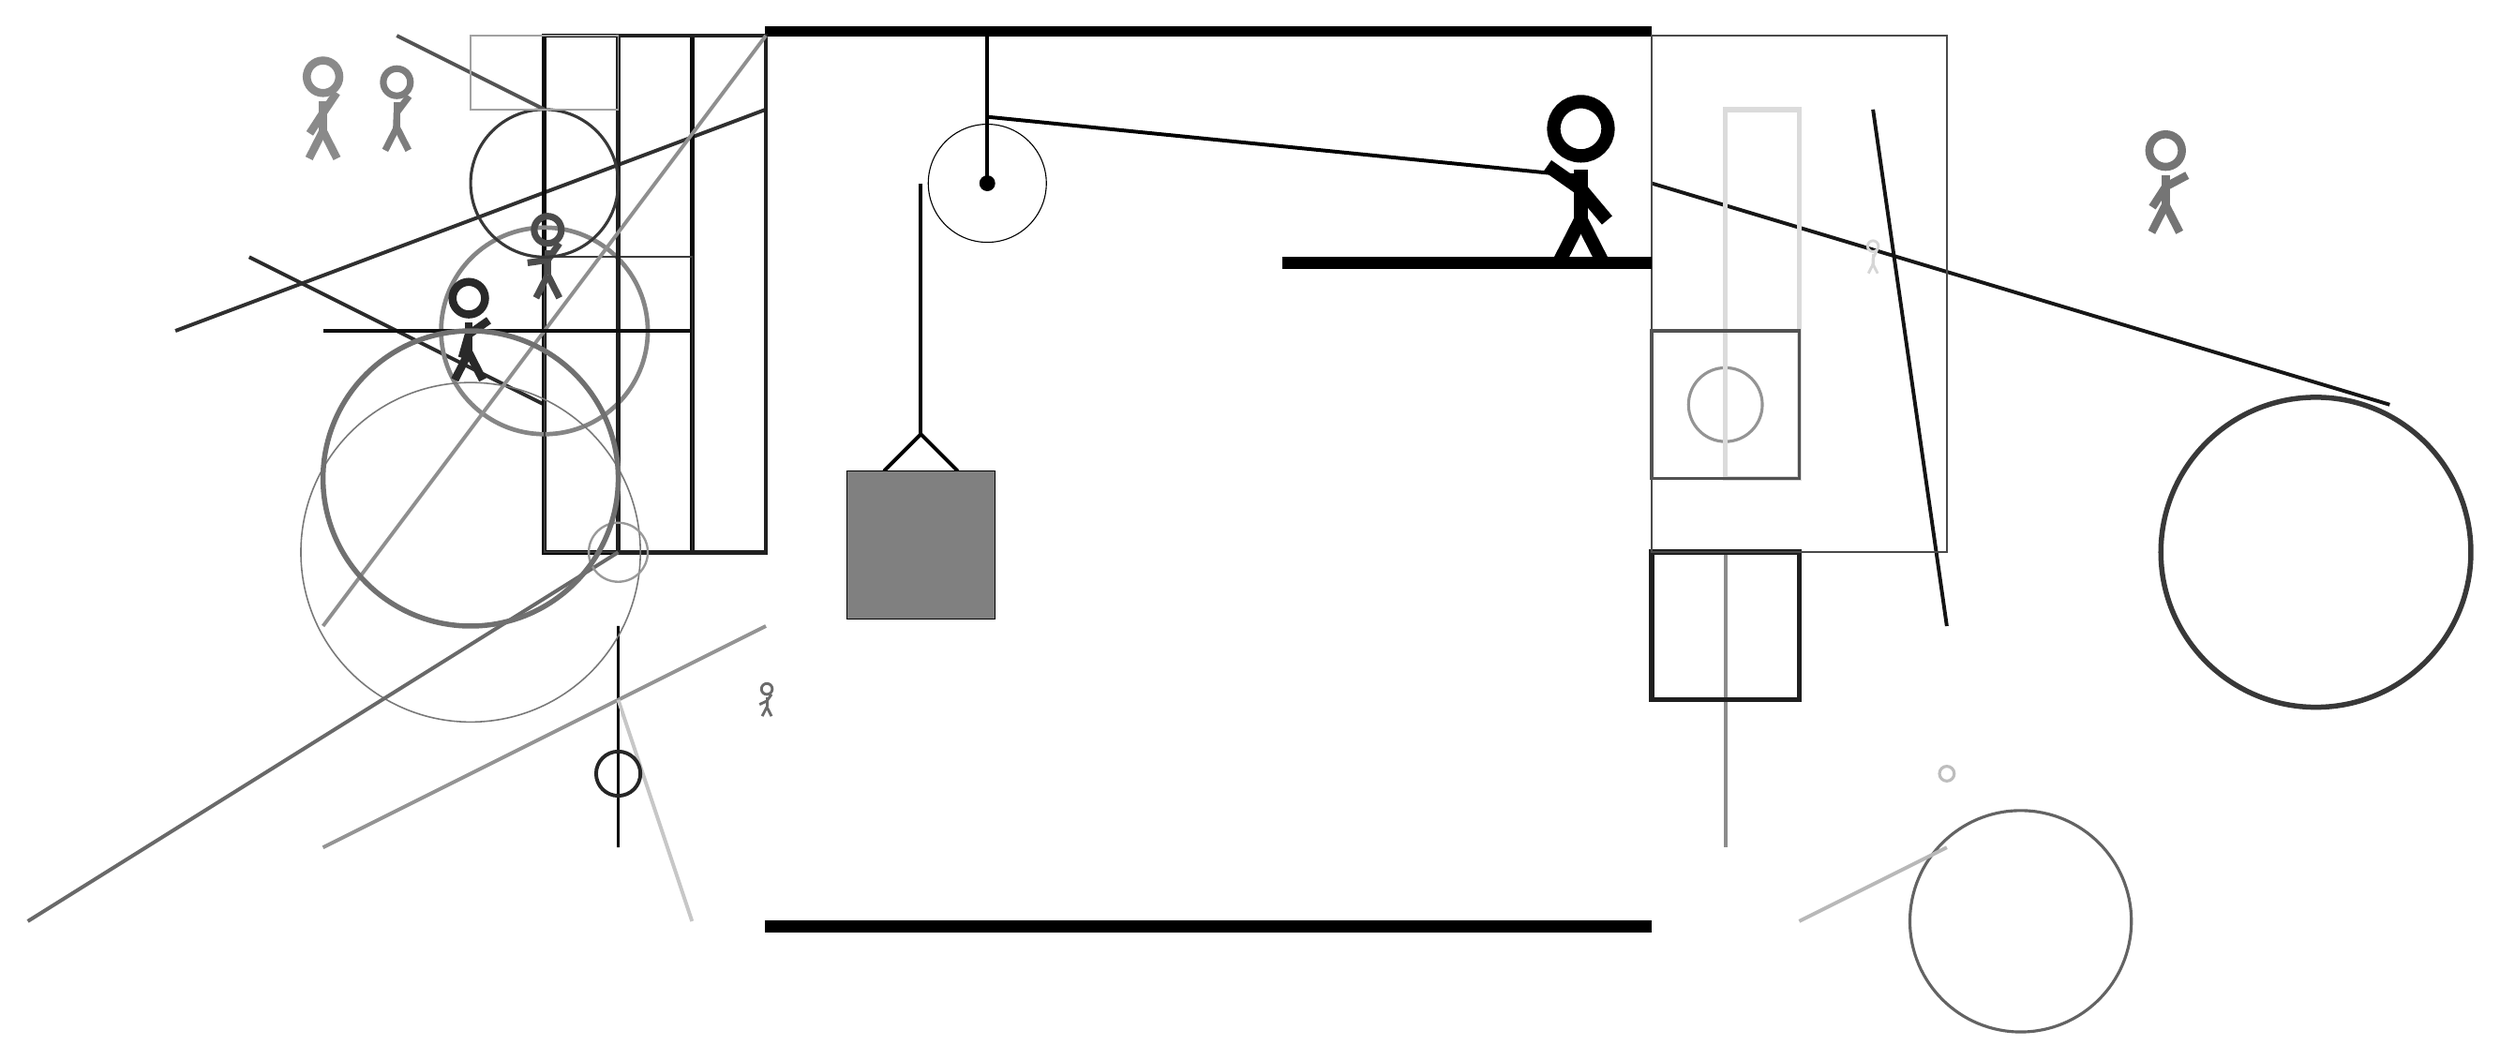
\begin{tikzpicture}
			%%%%% START %%%%%
			
			\draw[fill=black] (-2, 9) rectangle (10, 9.125);
			
			\draw (1, 7) circle (0.8);
			\draw[fill=black] (1, 7) circle (0.1);
			\draw[line width=0.5mm] (1, 9) -- (1, 7);
			
			\draw[line width=0.5mm](-0.4, 3.1) --  (0.1, 3.6) -- (0.6, 3.1);
			\draw[fill=black!50] (-0.9, 3.1) rectangle (1.1, 1.1);
			
			\draw[line width=0.5mm](0.1, 7) -- (0.1, 3.6);
			\centerarc[line width=0.5mm](1, 7)(90:180:0.9)
			\draw[line width=0.5mm](1, 7.9) -- (9, 7.1);
			
			\draw[line width=0.5mm, color=black!83](-5, 4) -- (-9, 6);
			
			\draw[line width=0.5mm, color=black!81](-2, 8) -- (-10, 5);
			\draw[line width=0.6mm, color=black!96] (-3, 2) rectangle (-5, 9);
			\draw [line width=0.6mm, color=black!48](-5, 5) circle (1.4);
			\draw[line width=0.5mm, color=black!91](10, 7) -- (20, 4);
			
			\draw[line width=0.2mm, color=black!77] (-3, 6) rectangle (-5, 2);
			\draw[line width=0.2mm, color=black!41] (-2, 9) rectangle (-2, 3);
			\draw[line width=0.6mm, color=black!87] (-2, 9) rectangle (-4, 2);
			\draw[line width=0.4mm, color=black!99] (-4, 1) rectangle (-4, -2);
			
			\draw [line width=0.4mm, color=black!42](11, 4) circle (0.5);
			
			\draw[line width=0.5mm, color=black!42](-2, 1) -- (-8, -2);
			\draw[line width=0.5mm, color=black!45](11, 2) -- (11, -2);
			\draw[line width=0.7mm, color=black!14] (12, 3) rectangle (11, 8);
			
			\node[line width=0.3mm, color=black!70] at (-5, 6) {\Strichmaxerl[5][8][55]};
			\node[line width=0.6mm, color=black!54] at (17, 7) {\Strichmaxerl[6][57][28]};
			\draw [line width=0.2mm, color=black!53](-6, 2) circle (2.3);
			\draw[line width=0.5mm, color=black!44](-2, 9) -- (-8, 1);
			\draw[line width=0.5mm, color=black!94](-3, 5) -- (-8, 5);
			\draw[line width=0.5mm, color=black!92](14, 1) -- (13, 8);
			\draw [line width=0.4mm, color=black!61](15, -3) circle (1.5);
			\draw[line width=0.5mm, color=black!22](-4, 0) -- (-3, -3);
			
			\node[line width=0.2mm, color=black!16] at (13, 6) {\Strichmaxerl[2][88][63]};
			
			\draw[line width=0.7mm, color=black!88] (12, 2) rectangle (10, 0);
			\draw[line width=0.5mm, color=black!28](14, -2) -- (12, -3);
			\node[line width=0.2mm, color=black!58] at (-2, 0) {\Strichmaxerl[2][25][55]};
			
			\node[line width=0.4mm, color=black!84] at (-6, 5) {\Strichmaxerl[6][74][35]};
			\draw[line width=0.3mm, color=black!71] (10, 9) rectangle (14, 2);
			\draw [line width=0.4mm, color=black!78](-5, 7) circle (1.0);
			
			\draw [line width=0.7mm, color=black!78](19, 2) circle (2.1);
			\draw[line width=0.4mm, color=black!68] (10, 3) rectangle (12, 5);
			\draw [line width=0.4mm, color=black!48](-5, 7) circle (0.0);
			
			\node[line width=0.7mm, color=black!46] at (-8, 8) {\Strichmaxerl[6][57][56]};
			\draw[line width=0.5mm, color=black!59](-4, 2) -- (-12, -3);
			\draw [line width=0.3mm, color=black!40](-4, 2) circle (0.4);
			\draw [line width=0.5mm, color=black!85](-4, -1) circle (0.3);
			\node[line width=0.5mm, color=black!51] at (-7, 8) {\Strichmaxerl[5][88][53]};
			
			\draw [line width=0.7mm, color=black!56](-6, 3) circle (2.0);
			
			\draw[line width=0.5mm, color=black!67](-7, 9) -- (-5, 8);
			\draw [line width=0.4mm, color=black!26](14, -1) circle (0.1);
			\draw[line width=0.2mm, color=black!37] (-4, 8) rectangle (-6, 9);
			
			\node at (9, 7) {\Strichmaxerl[10][-35][-50]};
			\draw[fill=black] (5, 6) rectangle (10, 5.85);
			
			\draw[fill=black] (-2, -3) rectangle (10, -3.15);
			
			%%%%% END %%%%%
		\end{tikzpicture}
	\end{figure}	
\end{document}